\documentclass[12pt]{article}
\usepackage[margin=1.0in]{geometry} %page layout
\usepackage[usenames,dvipsnames]{color} %color
\definecolor{light-gray}{gray}{0.95}
\definecolor{darkgreen}{rgb}{0,0.4,0}
\usepackage{graphicx, subfigure} %figures
\usepackage{url, hyperref} %cross-referencing
\usepackage{amsmath, amssymb} %math
\usepackage{listings} %source code
\lstset{breaklines=true,
breakindent=0pt,
prebreak=\mbox{\tiny$\searrow$},
postbreak=\mbox{{\color{blue}\tiny$\rightarrow$}},
numbers=left,
commentstyle=\color{darkgreen},
numberblanklines=false,
frame=single,
captionpos=b,
backgroundcolor=\color{light-gray}}
\usepackage[3D]{movie15} %for movies (needs hyperref)
	\newenvironment{changemargin}[2]
	{
	  	\begin{list}{}
		{
			\setlength{\topsep}{0pt}%
			\setlength{\leftmargin}{#1}%
			\setlength{\rightmargin}{#2}%
			\setlength{\listparindent}{\parindent}%
			\setlength{\itemindent}{\parindent}%
			\setlength{\parsep}{\parskip}%
		}
	  	\item[]
		}
		{\end{list}
	}
\author{Salman Aslam\\Georgia Tech}
\title{Particle Filter}
\date{}
\begin{document}
\maketitle
\rule[0pt]{\textwidth}{1pt}
\tableofcontents
\rule[0pt]{\textwidth}{1pt}

%=========================
\section{Goal}
%=========================
Track targets under the following conditions:

\begin{itemize}
\item Target dynamics are non-linear
\item Target dynamics are non-Gaussian
\item Online processing is required
\end{itemize}


%=========================
\section{Introduction}
%=========================
In the state-space approach to time series modeling, the focus is on the \emph{state vector} and its transition from state to state.  In tracking applications, the state vector could correspond to target dynamics.  In economic systems, the state vector could be composed of quantities such as inflation rates, currency exchange rates, inflation, etc.  In weather forecasting, the state vector could be based on hurricane speed, direction and strength.  It is clear that a large range of applications can be modeled using this approach.  However, in most cases, it is difficult to accurately estimate the states.  Noise induced by natural phenomena or erroneous observation can corrupt measurement of the state vector.  A noisy \emph{measurement vector} therefore relates observations to states.

In many cases, the state vector evolution can be modeled as a linear system,

\begin{align}
\mathbf{x}[k] &= \mathbf{A}\mathbf{x}[k-1] +  \mathbf{B}\mathbf{u}[k]\\
\mathbf{z}[k] &= \mathbf{A}\mathbf{x}[k] +  \mathbf{v}[k]\\
\end{align}

In such cases, One such example is given in Figure~\ref{TRK_overviewDiagram}.  

								\begin{figure}[t]
								\center
								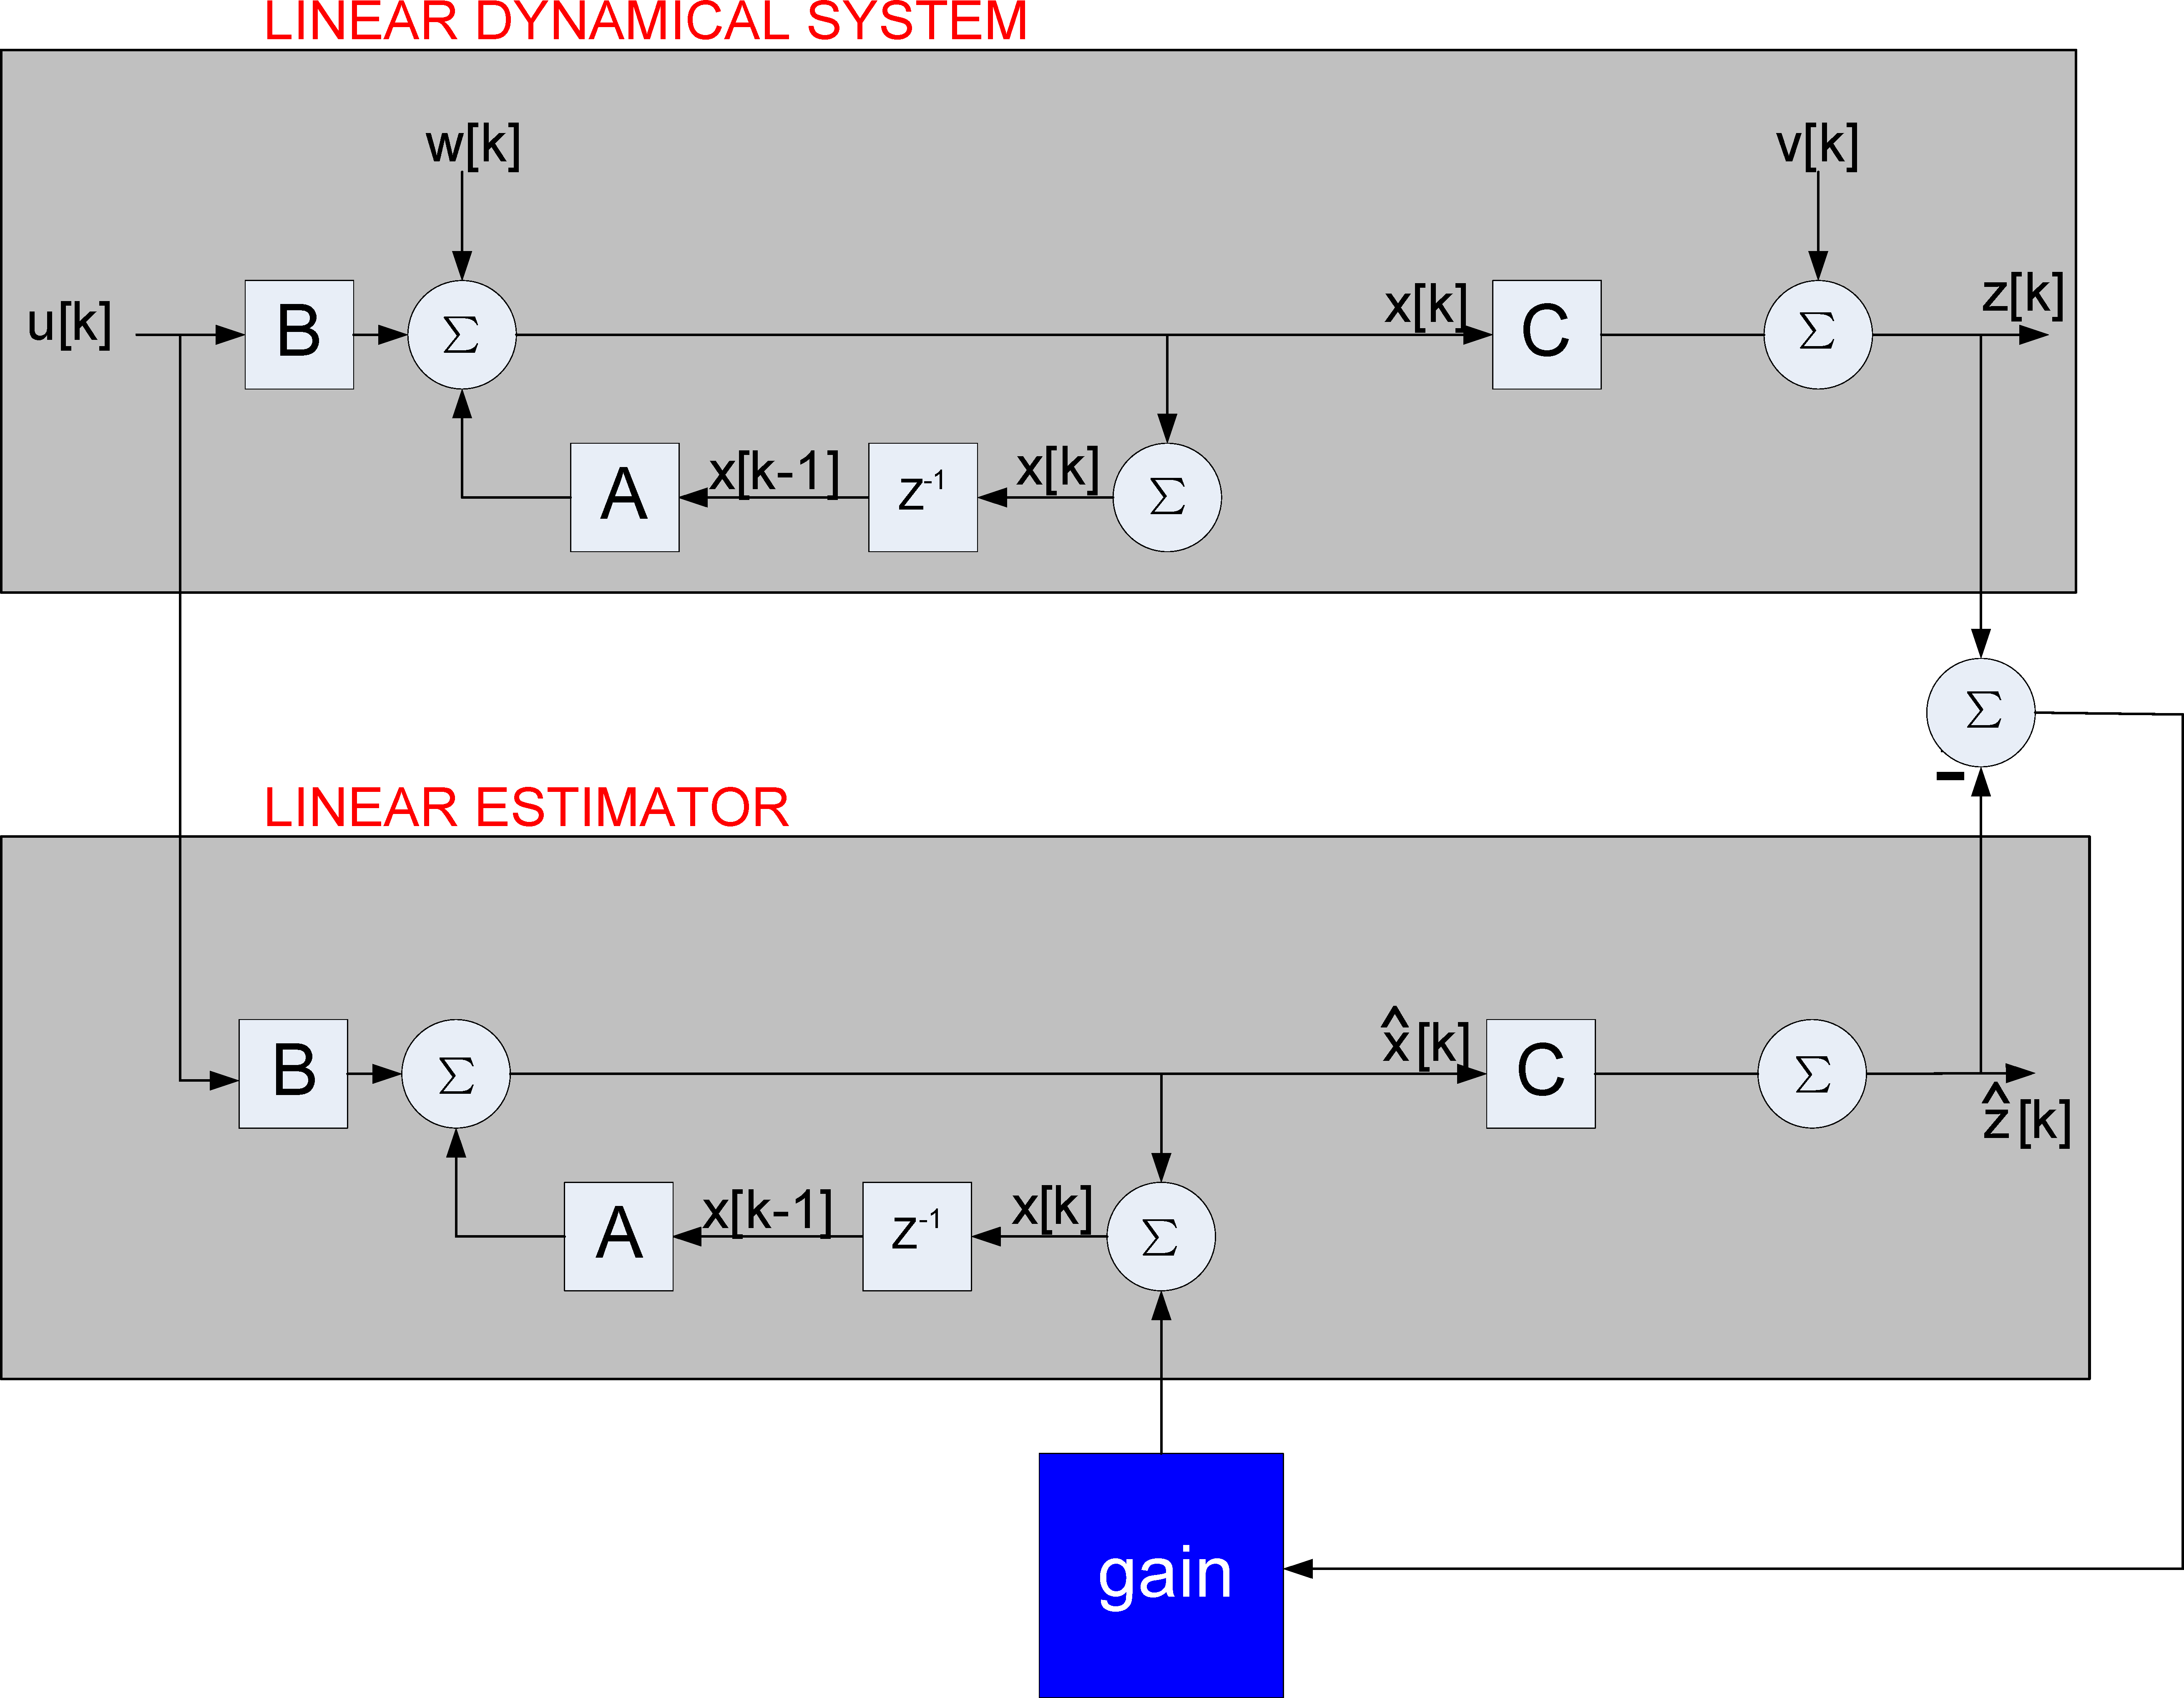
\includegraphics[width=1.0\textwidth]{figs/TRK_LinearEstimator_blockDiagram.pdf}
								\caption{Linear estimator.}
								\label{TRK_overviewDiagram}
								\end{figure}


The inference model in this work is based on a sequential Monte Carlo (SMC) filter, the particle filter.  The particle filter has been discussed in Chapter~\ref{chap_TRK}.  Almost all particle filters are based on the sequential importance sampling (SIS) algorithm, including the sampling importance resampling (SIR) filter, auxiliary sampling importance resampling (ASIR) filter and the regularized particle filter (RPF).  The basic difference between these algorithms is the choice of \emph{importance sampling density} and/or modification of the resampling step~\cite{2002_JNL_PF_Arulampalam}.  

In this work, we use the basic SIS algorithm.  It is essentially the same as the SIR filter except that there is no resampling step.  However, like the SIR filter, we use the prior density as the importance sampling density.  The weights on the posterior are computed using the appearance model for PCA, RVQ or TSVQ, depending on which of these algorithms is being used.  For RVQ for instance, the mean squared reconstruction error is used for the weighting.

%=========================
\section{Theory}
%=========================




A commonly used formulation for tracking is based on Bayesian estimation.  In this framework, target kinematics are modeled as the latent states of a time-dynamic system~\cite{2002_JNL_PF_Arulampalam}.  Time-dynamic systems are based on two models: (a) \emph{state prediction model}, ${f_t:R^D \times R^D \rightarrow R^D}$, describing state evolution, and (b) \emph{observation model}, ${h_t:R^N \times R^N \rightarrow R^N}$, relating observations to the states.  These models are described as,

\begin{align}
\mathbf{x}_t &= f_t(\mathbf{x}_{t-1}, \mathbf{v}_{t-1}) \notag\\
\mathbf{z}_t &= h_t(\mathbf{x}_t, \mathbf{n}_t)
\label{Eq:TDS}
\end{align}

$\mathbf{v} \in R^D$ is an independent, identically-distributed (IID) process noise sequence.  $\mathbf{n} \in R^N$ is an IID measurement noise sequence.  The goal is to find the estimate of the state $\mathbf{x}_t$ at time $t$, based on all observations $\mathbf{Z}_t={\{\mathbf{z}_i, i=1,...,T\}}$.   $\mathbf{z}_t$ is the observation vector at time $t$.  

At this point, it is interesting to place the process of tracking in the bigger picture of probabilistic graphical models, as shown in Figure~\ref{fig:TRK_big_picture}.  Mathematically, hidden Markov models (HMMs) can also be written using evolution and observation models even though the method was developed independently of time dynamic systems \cite{2007_BOOK_PRML_Bishop}.  

This two stage model lends itself well to Bayesian inference \cite{2002_JNL_PF_Arulampalam}.  The reason is that observations can be used as evidence to modulate the prior distribution on the states.  We can then infer the posterior distribution on the states using Bayes' Rule.  Mathematically, the Chapman Kolmogorov equation predicts the next state by combining information from the state prediction model $p(\mathbf{x}_t| \mathbf{x}_{t-1})$ and all previous observations $\mathbf{Z}_{t-1}$.  %This is given in Equation~\ref{Eqn:TRK_prediction}.

{%\Large
\begin{equation}
\begin{array}{lllllllll}
{\color{darkgreen}p(x_t|Z_{t-1})} &= \frac{p(x_t, Z_{t-1})}{p(Z_{t-1})}\\
&=\frac{\int p(x_t, x_{t-1}, Z_{t-1})dx_{t-1}}{p(Z_{t-1})}\\
&=\frac{\int {\color{Cyan}p(x_t|x_{t-1}, Z_{t-1})}p(x_{t-1},Z_{t-1})dx_{t-1}}{p(Z_{t-1})}\\
&=\frac{\int {\color{Cyan}p(x_t|x_{t-1})}{\color{red}p(x_{t-1}|Z_{t-1})}p(Z_{t-1})dx_{t-1}}{p(Z_{t-1})}\\
&=\int {\color{Cyan}p(x_t|x_{t-1})}{\color{red}p(x_{t-1}|Z_{t-1})}dx_{t-1}
\end{array}
\label{Eqn:TRK_prediction}
\end{equation}
}


%\begin{equation}
%p(x_k|\textbf{Z}_{k-1})=
%\int{p(\mathbf{x}_k| \mathbf{x}_{k-1})p(\mathbf{x}_{k-1}|\mathbf{Z}_{k-1})}d\mathbf{x}_{k-1}
%\label{eq:ChapmanKolmogorov}
%\end{equation}  

In the second step, the observation $\mathbf{z}_t$ at time $t$ and the predicted state $\mathbf{x}_t$ can be used to compute the posterior estimate of the state $\mathbf{x}_t$ using %Equation~\ref{Eqn:TRK_update}.


{%\large
\begin{equation}
\begin{array}{lllllllll}
{\color{red}p(x_t | Z_t)} &= \frac{p(x_t, Z_t)}{p(Z_t)}\\
&= \frac{p(x_t, z_t, Z_{t-1})}{p(z_t, Z_{t-1})}\\
&= \frac{{\color{blue}p(z_t|x_t,Z_{t-1})}p(x_t, Z_{t-1})}{p(z_t|Z_{t-1})p(Z_{t-1})}\\
&= \frac{{\color{blue}p(z_t|x_t)}{\color{darkgreen}p(x_t|Z_{t-1})}p(Z_{t-1})}{p(z_t|Z_{t-1})p(Z_{t-1})}\\
&= \frac{{\color{blue}p(z_t|x_t)}{\color{darkgreen}p(x_t|Z_{t-1})}}{\int{p(z_t|x_t){\color{darkgreen}p(x_t |Z_{t-1})}}dx_t}
\end{array}
\label{Eqn:TRK_update}
\end{equation}
}



%\begin{equation}
%p(\mathbf{x}_k|\textbf{Z}_k)	= \frac{p(\mathbf{z}_k|\mathbf{x}_k)p(\mathbf{x}_k |\textbf{Z}_{k-1})   }{p(\mathbf{z}_k| \textbf{Z}_{k-1})}
%\label{eq:posterior}			
%\end{equation}

Equations~\ref{Eqn:TRK_prediction} and~\ref{Eqn:TRK_update} form the optimal Bayesian solution for the recursive propagation of the posterior density.  This problem can be solved analytically using the closed-form Wiener-Kalman linear Minimum Mean Square Estimate (MMSE) in Gaussian noise \cite{1964_JNL_BayesianEstimation_Ho, 1993_BOOK_SSP_Kay}.  Non-analytical methods, such as grid-based methods, can be used if the state space is discrete and consists of a finite number of states.  For non-linear models, the Extended Kalman Filter (EKF) computes the Jacobian for a Taylor Series expansion of the system and observation models about the current state \cite{2005_Misc_KalmanFilterComparison_Orderud}.  Recently, the Unscented Kalman Filter (UKF) has been replacing the EKF in a wide range of applications.  The UKF, instead of explicitly computing the Jacobian, computes a set of points that capture the true mean and covariance of the prior.  When propagated through the non-linear system, these points capture the posterior mean and covariance \cite{1997_CNF_UKF_Julier}.  As a result, the UKF estimates the posterior mean and covariance accurately to at least the second-order Taylor Series expansion.  The EKF on the other hand achieves only first-order accuracy \cite{2004_CNF_SigmaPointKalman_Merwe, 2000_CNF_UKF_Wan}.  More recently, particle filters which use point mass representations for probability densities and are based on stochastic sampling have been introduced in the visual tracking literature \cite{1993_JNL_ParticleFilter_Gordon, 2001_JNL_PFjumpMarkov_Doucet}.  A primary difference between the UKF and the particle filter is that the former is based on deterministic sampling while the latter is based on stochastic sampling.  Particle filters offer an additional advantage of being able to handle arbitrary densities as shown in Figure~\ref{fig:particle_filter_multi_modal_density}.  However, since the particle filter uses non-parametric densities with no functional representations, its computations do not scale well as the dimensionality increases~\cite{2004_CNF_TrackingPeople_Zhao}.  

A variety of particle filters have now been introduced.   According to~\cite{2002_JNL_PF_Arulampalam}, sequential Monte Carlo (SMC) filtering has been called particle filtering~\cite{1999_CNF_PF_carpenter}, bootstrap filtering~\cite{1993_JNL_ParticleFilter_Gordon}, the condensation algorithm~\cite{1998_JNL_Condensation_IsardBlake}, interacting particle approximations~\cite{1999_JNL_PF_Crisan, 1999_BK_PF_Moral} and survival of the fittest~\cite{1995_CNF_PF_Kanazawa}.

  
%The particle filter formulation is generally similar to the method which is used for the Kalman Filter.  A prediction step is followed by an update step, which is followed by a prediction step, and so on.  The update equation at time $t$ for a state $x_t$ given all observations $z_T$ involves computing the posterior density $p(x_t | Z_t)$.  In this case, the posterior density factors into a likelihood at time $t$, $p(z_t|x_t)$ and a prior density, $p(x_t|Z_{t-1})$, 
%
%
%
%
%The prior density can be computed using the Chapman-Kolmogorov equation by introducing the nuisance parameter $x_{t-1}$,
%
%
%$p(x_t|x_{t-1})$ is computed using the motion model while $p(x_{t-1}|Z_{t-1})$ is the posterior density from the previous time step, $t-1$.
%
%
%Visual tracking in clutter is difficult using the Kalman filter since clutter can typically give rise to several competing observations which encourage a non-unimodal density and gaussian densities cannot represent simultaneous alternative hypotheses~\cite{1998_JNL_Condensation_IsardBlake}.  Moreover 


%However, currently, the most popular version is the SIR (Sampling Importance Resampling) filter \cite{2009_BOOK_PF_Doucet}.  The resampling step prevents the posterior from collapsing to a single point.  The steps involved in computing the solution to this filter are summarized below:

%\begin{itemize}
%\item \textbf{Sampling with replacement.}  This step is carried out to guarantee that the algorithm runs within given computational resources.  $N$ samples are chosen from the set $\mathbf{s}_{k-1}^n$, each element being chosen with probability $\pi_{k-1}^n$.  %a sampling with replacement st from $p(\mathbf{x}_k | \mathbf{x}_{k-1})$
%\item Calculate particle weights from the likelihood, $\mathbf{w}_k = p(\mathbf{z}_k|\mathbf{x}_k)$
%\item Calculate the posterior ($p(\mathbf{x}_k | \mathbf{x}_{k-1})$.  First normalize weights.  Then resample using normalized-weights and sampled-prior. 
%\end{itemize}
The density to be resampled is called the test density.


								\begin{figure}[t]
								\centering
								\subfigure[Reference (uniform) density and test PDF.]{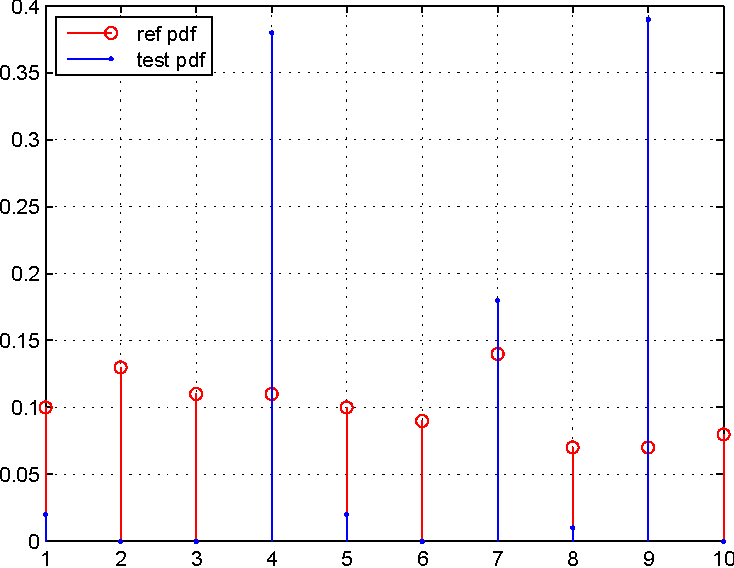
\includegraphics[width=0.4\textwidth]{figs/particle_filter_pdfs.pdf}}
								\subfigure[Comparing CDFs.]{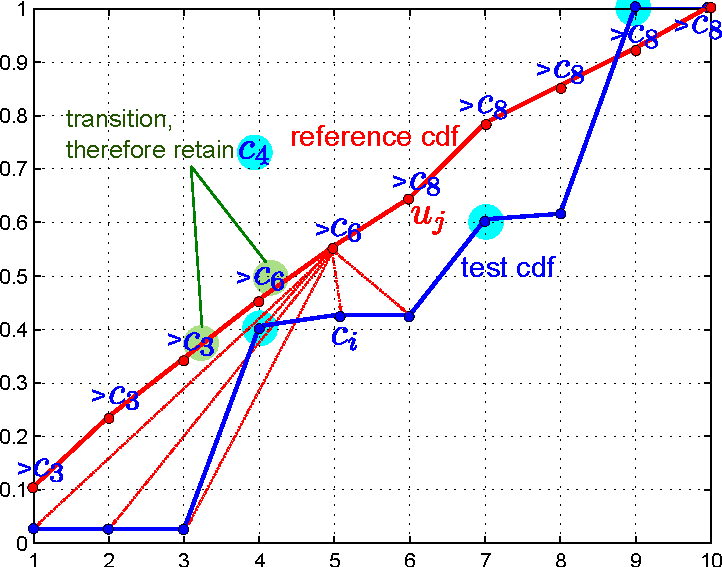
\includegraphics[width=0.4\textwidth]{figs/particle_filter_resampling.pdf}}
								\subfigure[Particles 4, 7 and 9 are picked repeatedly since they have higher weight.]{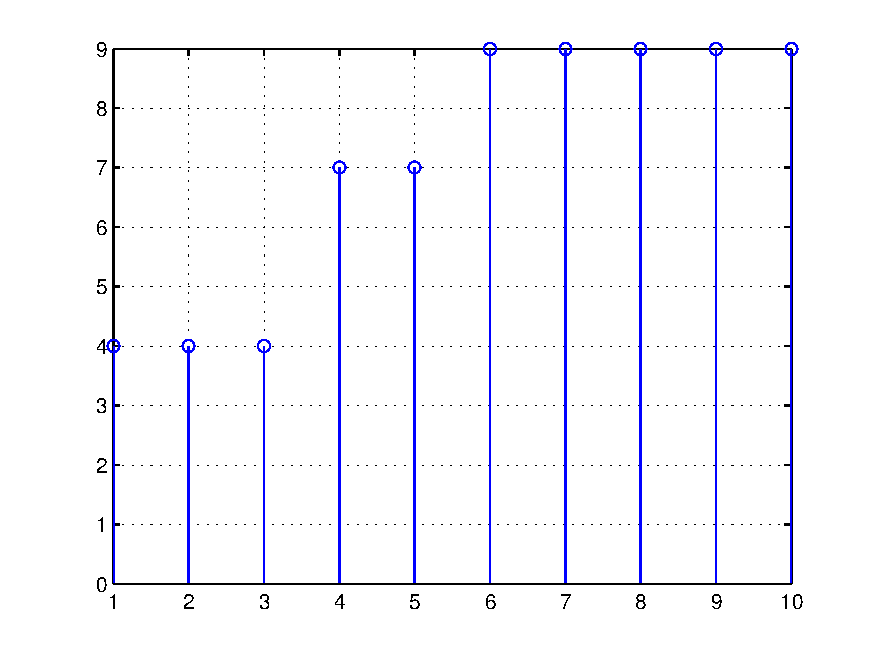
\includegraphics[width=0.45\textwidth]{figs/particle_filter_particles.pdf}}
								\subfigure[Resampled PDF.]{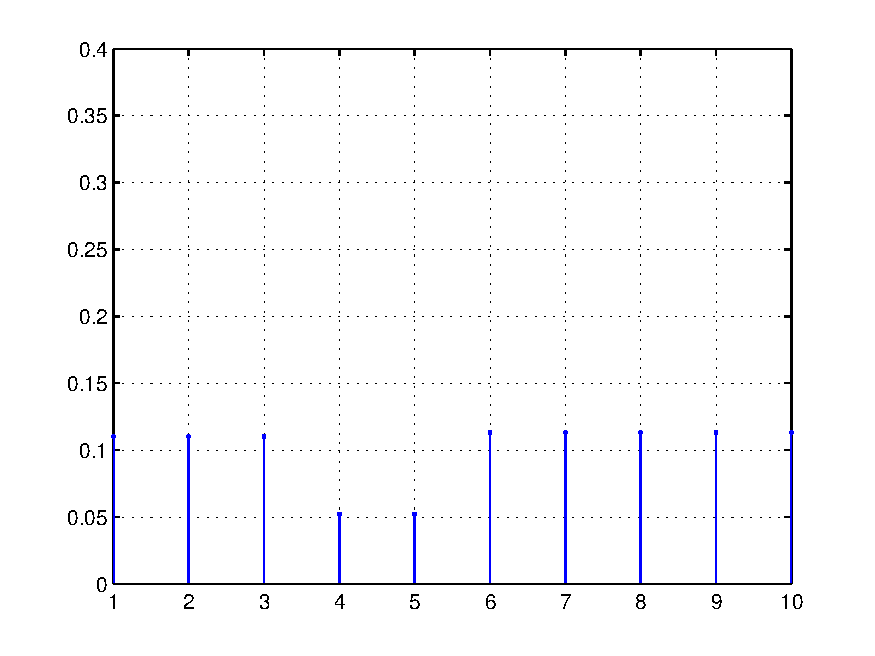
\includegraphics[width=0.45\textwidth]{figs/particle_filter_resampled_density.pdf}}
								\caption{Particle filter, resampling.  Source code for this is given in Listing~\ref{lst:main_TRK_particle_filter_resampling} and~\ref{lst:TRK_particle_filter_resampling}}.   
								\label{fig:particle_filter_resampling}
								\end{figure}
								

\section{Resampling}
Samples are generated from a uniform density.  The CDF of this reference density is then compared with the CDF of the test density.  This is shown in Figure~\ref{fig:particle_filter_resampling}.  Each value of the reference density is compared with values of the test density.  

\newpage
\tiny
\appendix
\section{Source code}
\subsection{Resampling}
\lstinputlisting[caption={main\_TRK\_particle\_filter\_resampling.m.}, 						label=lst:main_TRK_particle_filter_resampling]						{main_TRK_particle_filter_resampling.m}
\lstinputlisting[caption={TRK\_particle\_filter\_resampling.m.}, 								label=lst:TRK_particle_filter_resampling]								{TRK_particle_filter_resampling.m}

\normalsize
\bibliographystyle{ieee}
\bibliography{MyCitations}
\end{document}